\documentclass[conf]{new-aiaa}
%\documentclass[journal]{new-aiaa} for journal papers
\usepackage[utf8]{inputenc}

\usepackage{graphicx}
\usepackage{amsmath}
\usepackage[version=4]{mhchem}
\usepackage{siunitx}
\usepackage{longtable,tabularx}
\usepackage{float}
\usepackage{subfigmat}
\usepackage{setspace}
\doublespacing

\setlength\LTleft{0pt} 

\title{Vector field  path following and obstacle avoidance singularity mitigation via look-ahead flight envelope}

\author{First A. Author\footnote{Insert Job Title, Department Name, Address/Mail Stop, and AIAA Member Grade (if any) for first author.} and Second B. Author Jr.\footnote{Insert Job Title, Department Name, Address/Mail Stop, and AIAA Member Grade (if any) for second author.}}
\affil{Business or Academic Affiliation 1, City, State, Zip Code}
\author{Third C. Author\footnote{Insert Job Title, Department Name, Address/Mail Stop, and AIAA Member Grade (if any) for third author.}}


\begin{document}

\maketitle

\begin{abstract}
Unmanned Aerial Vehicles (UAVs) conventionally navigate by following a series of pre-planned waypoints generated off-line, which are initially obstacle free, may be to be re-planned when encountering previously unknown obstacles. Re-planning waypoints could be avoided by implementing a path following and obstacle avoidance vector field guidance. Convergent vector fields attract a UAV to follow a path while repulsive vector fields push the UAV away from no-fly zones. Combining attractive and repulsive fields may cause small regions of null guidance, called singularities, which may be avoided by tuning vector field parameters. 
\end{abstract}
%Unmanned Aerial Vehicles (UAVs) conventionally navigate a series of off-line generated and initially obstacle free waypoints that may have to be re-planned when encountering a previously unknown obstacle. Re-planning waypoints could be avoided by implementing a path following and obstacle avoidance vector field guidance. Guidance to converge and follow a pre-planned path is produced by an attractive vector field while obstacles are represented by a repulsive vector field. Summing together attractive goal and repulsive obstacle fields produce a guidance for tracking a pre-planned path while avoiding unplanned obstacles. Small regions of null guidance, called singularities, may be produced when summing attractive and repulsive fields together. 





 

%\textbf{Motivation}
%\begin{itemize}
%	\item Conventional waypoint guidance relies on a pre-planned, flyable, and obstacle free path 
%	\item Obstacles unaccounted for during planning may require a re-plan which may require communication with a ground station
%\end{itemize}
%
%
%\textbf{Background}
%\begin{itemize}
%	\item Vector field guidance for path following has been shown to be both robust in the presence of external disturbances and produce low cross track error flight
%	\item Obstacles can be represented as repulsive fields and summed with attractive fields to produce an obstacle avoidance guidance
%	\item  Summing vector field guidance my produce singularities, resulting in no guidance
%	\item Repulsive fields currently provide no additional information on how to go around obstacle
%\end{itemize}
%
%
%\textbf{Contribution}
%\begin{itemize}
%	\item Method for compensating for singularities that may be experienced (Lookahead or fast detection)
%\end{itemize}




\section{Nomenclature}

{\renewcommand\arraystretch{1.0}
\noindent\begin{longtable*}{@{}l @{\quad=\quad} l@{}}
$UAV$  & Unmanned Aerial Vehicle \\
$VF$   & Vector Field \\
$VFF$  & Virtual Force Field \\
$LVF$  & Lyapunov Vector Field \\
$GVF$  & Goncalves Vector Field \\
\end{longtable*}}

\section{Introduction}
Unmanned Aerial Vehicles are pilotless aircraft used by military, police, and civilian communities for tasks such as reconnaissance, damage assessment, natural disaster surveying, and target tracking \cite{ariyur_autonomous_2008,teuliere_chasing_2011}. Tasks can be performed by a single UAV or with a team of other air, ground, or marine vehicles \cite{oh_coordinated_2013,hyondong_oh_coordinated_2015,ulun_coordinated_2013}. Autonomous vehicle missions are typically accomplished by navigating a series of waypoints \cite{ariyur_autonomous_2008} or path following \cite{oliveira_moving_2016}. Waypoints are conventionally generated off-line at a ground station and relayed over radio to the UAVs autopilot. Obstacles such as buildings, terrain, and other vehicles can be avoided by planning waypoints around obstacles. The on-board guidance directs the UAV towards the current active waypoint, once the UAV has reached a pre-defined distance from the waypoint the UAV is directed to the next waypoint. An example of a UAV following waypoint guidance while avoiding an obstacle is shown in Figure \ref{fig:simplewaypointsWithUAVPath}


\begin{figure}[H]
	\centering
	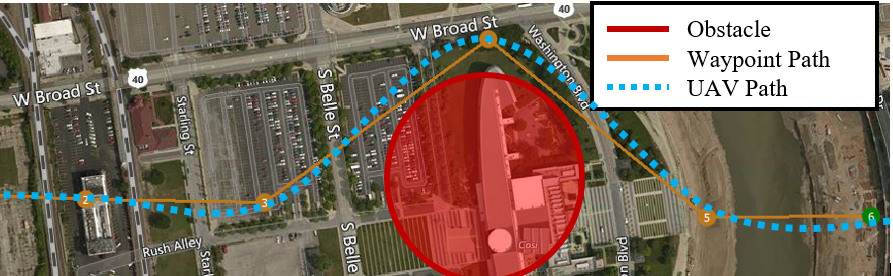
\includegraphics[width=1\linewidth]{Figures/simpleWaypointsWithUAVPath}
	\caption{UAV path from waypoint guidance}
	\label{fig:simplewaypointsWithUAVPath}
\end{figure}


During waypoint navigation the UAV may encounter obstacles or environmental changes that would require a new set of obstacle free waypoints to be generated. For highly uncertain or dynamic environments, there may have to be frequent updates which increases the communication overhead of the autopilot. Additionally, if communication is delayed or lost, waypoints may not be updated rapidly enough and the UAv may fail to avoid the obstacles.


Obstacle free paths in static and dynamic environments have been generated with the potential field method, which models a robot's workspace as a gradient of artificial attractive and repulsive forces \cite{khatib_real-time_1986}. Potential field combines path planning, trajectory planning, and control into a single system \cite{rimon_exact_1992} making it an attractive solution path planning. Paths can be generated by placing a point mass at an initially high potential and allowing it to descend a gradient until the point reaches the goal, located at a global minimum potential. Obstacles provide a limited repulsive force, pushing the mass away from the obstacle. 


A histogram based potential field method can be found in \cite{borenstein_real-time_1990,borenstein_vector_1991,koren_potential_1991} which allowed for real time goal seeking with obstacle avoidance. Sensors on-board a ground robot located at $(x_0,y_0)$ detect obstacles within a pre-defined window containing a fixed number of cells. Cells containing an obstacle provide a repulsive force $\overrightarrow{F_{i,j}}$ opposite in direction to the line-of-sight from vehicle to cell location $(x_i,y_j)$, where $(i,j$) represents the cell index, $F_{cr}$ is a constant repulsive force, $W$ the vehicles width, $C_{i,j}$ a cells certainty, and $d_{i,j}$ the distance to the center of the cell with respect to robots center.

\begin{equation}\label{eq:vffRepulse}
\overrightarrow{F_{i,j}} = \frac{F_{cr}W^nC_{i,j}}{d^n_{i,j}} \bigg( \frac{x_i-x_0}{d_{i,j}}\hat{x} + \frac{y_i-y_0}{d_{i,j}}\hat{y}\bigg)
\end{equation}

The total repulsive force exerted on the robot is determined by summing the active cells, shown in Equation \ref{eq:vffRepulseSum}


\begin{equation}\label{eq:vffRepulseSum}
\overrightarrow{F_r} = \sum_{i,j}\overrightarrow{F_{i,j}}
\end{equation}

The robot is attracted to the goal by force $\overrightarrow{F_t}$ with constant magnitude $F_{ct}$ and along the LOS from robot center to goal, located at $(x_t,y_t)$ and a distance $d_t$, shown in Equation \ref{eq:vffGoal}

\begin{equation}\label{eq:vffGoal}
\overrightarrow{F_t} = F_{ct} \bigg( \frac{x_t-x_0}{d_{t}}\hat{x} + \frac{y_t-y_0}{d_{t}}\hat{y}\bigg)
\end{equation}

Summing together attractive and repulsive forces produces a vector that can be used for heading guidance, shown in Equation \ref{eq:vffHeading}

\begin{equation}\label{eq:vffHeading}
\overrightarrow{R} = \overrightarrow{F_r} + \overrightarrow{F_t}
\end{equation}

 Major drawbacks to potential field were identified in \cite{koren_potential_1991} consisting of local minimum and oscillations in corridors. The local minimum problem occurs when closely spaced obstacle's potential combine to produce a well on the descent gradient where a pre-mature stable point is found. Proposed solutions to local minimum include object clustering and virtual waypoint method \cite{liu_virtual-waypoint_2016}, virtual escaping route \cite{kim_escaping_2009}, and use of navigation functions \cite{goerzen_survey_2010}. Oscillations in potential field were studied in \cite{lei_tang_novel_2010}, and \cite{li_efficient_2012}.

In addition to local minimum and oscillations, potential field converges to a singular point which is not possible for fix wing aircraft. Similar to conventional waypoint guidance, the active goal point would change as a function of proximity. Simulating a UAV using VFF as guidance for a Dubins vehicle was performed and is shown in Figure \ref{fig:vffsimulated}, where a single obstacle cell located at the origin. The UAV initially travels directly toward the goal located at $(20,0)$ until the obstacle is encountered, at which point a repulsive force is applied. The UAV avoids the obstacle, however significantly deviates and fails to get back on the path between waypoints. For certain applications, such as following a curved ground track, surveying, or target following, it may be beneficial to follow an explicit path. 


\begin{figure}[H]
	\centering
	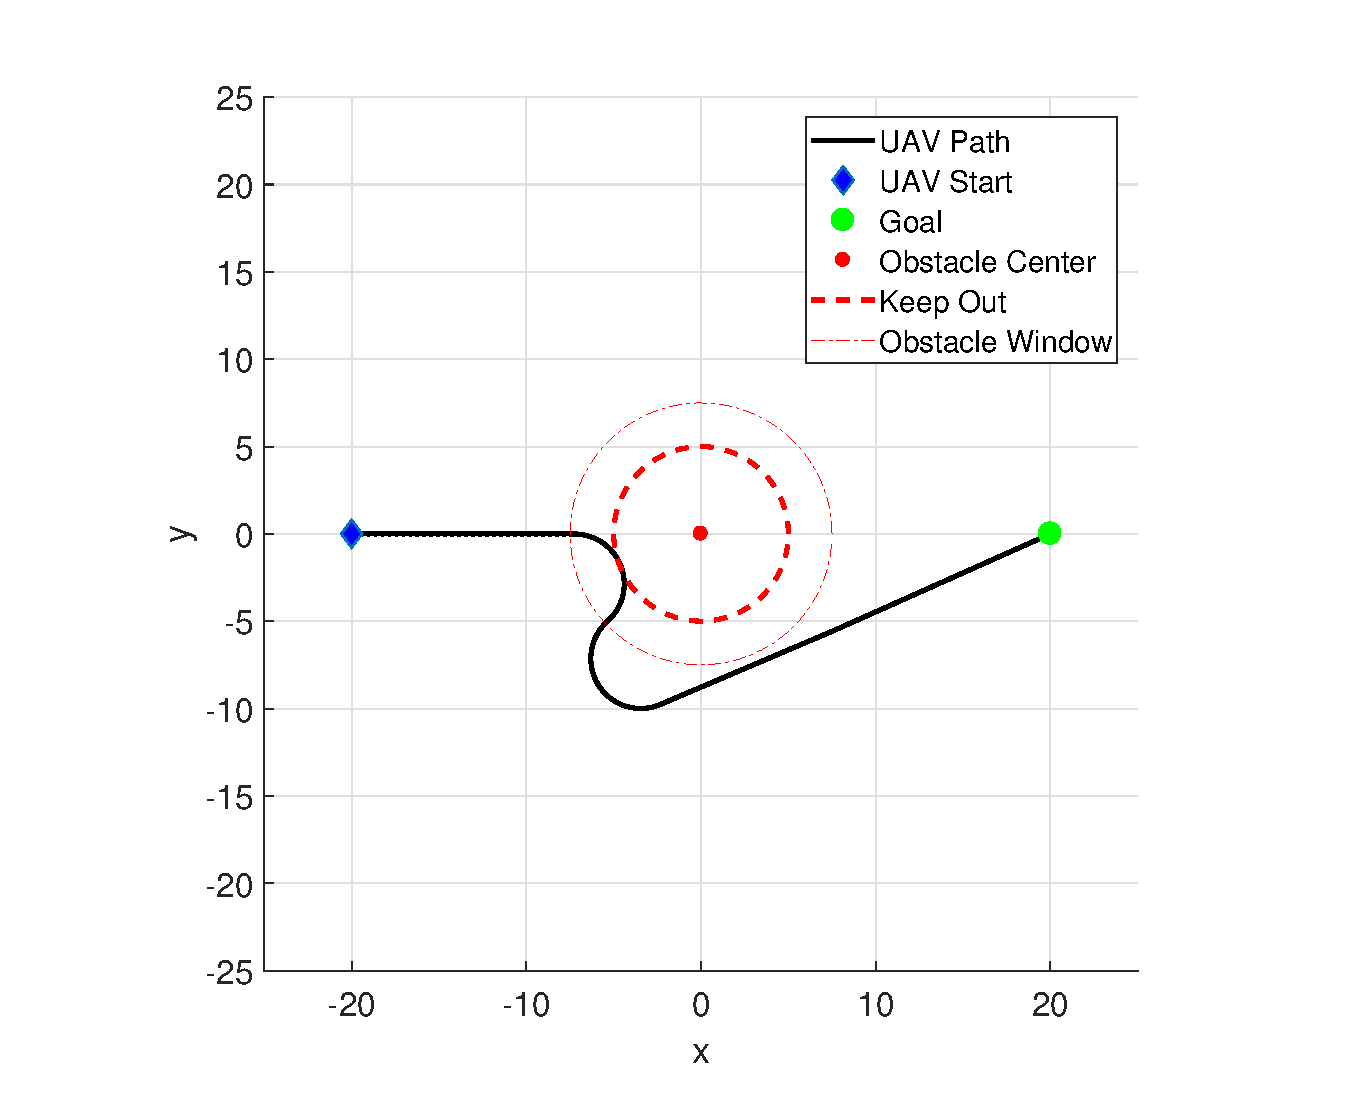
\includegraphics[width=0.7\linewidth]{Figures/vffSimulated}
	\caption{}
	\label{fig:vffsimulated}
\end{figure} 



% The potential field method converges to a singular point which is not possible for fixed wing aircraft. Similar to conventional waypoint guidance, the active goal point would change as a function of proximity, however for certain UAV applications such as following a curved ground track or surveying it may be beneficial to follow an explicit path. \\




%A robot at an initially high potential transitions down the gradient to a lower potential. Obstacles are represented by a high potential that act as repulsive forces.
%
%which operates on the principle of attractive and repulsive forces \cite{khatib_real-time_1986}. A robot at an initially high potential is pulled towards a goal located at a globally minimum potential while being repelled by obstacles in close proximity by repulsive forces.

 


%For highly uncertain or dynamic environments, there may have to be frequent updates which may not be possible if communication with the ground station is lost and may not
%
%
%During waypoint navigation the UAV may encounter an obstacle unknown during planning or experience a change in the environment which may require a new obstacle free series of waypoints be generated. A highly uncertain or dynamic environment would require frequent waypoint re-planning which may be difficult or impossible if communication with the ground station is lost. \\


 
%--- Potential Field Methods ----
%Potential field combines path planning, trajectory planning, and control into a single process \cite{rimon_exact_1992}  and is based on the principle of artificial attractive and repulsive forces \cite{khatib_real-time_1986}. 
%
%A robot at an initially high potential is pulled towards a goal located at a globally minimum potential while being repelled by obstacles in close proximity by repulsive forces.
%
% Major drawbacks to potential field were pointed out in \cite{koren_potential_1991} consisting of local minimum and oscillations in corridors. The local minimum problem occurs when closely spaced obstacle's potential combine to produce a well on the descent gradient where a pre-mature stable point is found. Proposed solutions to local minimum include object clustering and virtual waypoint method \cite{liu_virtual-waypoint_2016}, virtual escaping route \cite{kim_escaping_2009}, and use of navigation functions \cite{goerzen_survey_2010}. Oscillations in potential field were studied in \cite{lei_tang_novel_2010}, and \cite{li_efficient_2012}. \\

%The potential field method converges to a singular point which is not possible for fixed wing aircraft. Similar to conventional waypoint guidance, the active goal point would change as a function of proximity, however for certain UAV applications such as following a curved ground track or surveying it may be beneficial to follow an explicit path. \\
	
Such path following can be accomplished with vector fields which produce a heading guidance that asymptotically converges and circulates a path. A comparison between vector field and waypoint guidance techniques was presented in \cite{sujit_unmanned_2014} where each method was evaluated based on its complexity, robustness, and accuracy. Vector field produced guidance that was both robust to external wind disturbances while maintaining a low cross track error. \\


The two most prominent methods for generating vector fields in literature consist of the Lyapunov \cite{nelson_cooperative_2005,nelson_vector_2006,nelson_vector_2007,frew_cooperative_2007,miao_orthogonal_2016,griffiths_vector_2006} and Goncalves \cite{goncalves_artificial_2009,goncalves_circulation_2010,goncalves_vector_2010,gerlach_autonomous_2014} method. Lyapunov vector fields for converging and following straight and circular paths were described in \cite{nelson_cooperative_2005}. For converging and following a straight path, a guidance vector $\chi^{d}$ is determined in Equation \ref{eq:lyapunovStraight}, where $\chi^{\infty}$ is the course approach angle, $y$ is the lateral distance to the path, and $k$ is a positive constant that determines the rate of transition between convergence and following. An example of a Lyapunov vector field converging and following a straight line is shown in Figure \ref{fig:vfPrimitives}a.



% and are defined in Equations \ref{eq:lyapunovStraight} and \ref{eq:lyapunovCirc} respectively.

%------ Nelson VF equations -----
\begin{equation}\label{eq:lyapunovStraight}
\chi^d(y) = -\chi^{\infty}\frac{2}{\pi}\tan^{-1}(ky)
\end{equation}



For converging and following a circular path, a guidance vector $\chi^{d}$ is determined in Equation \ref{eq:lyapunovCirc}, where $\gamma$ is the UAVs angular position with respect to the circle, $r$ is the paths radius, $d$ is the distance from the circles center, and $k$ is a positive constant that determines the transition behavior. An example of a Lyapunov vector field for converging and following a circular \ref{fig:vfPrimitives}b.

\begin{equation}\label{eq:lyapunovCirc}
\chi^d(d) = \gamma-\frac{\pi}{2}-\tan^{-1} \bigg(k \frac{d-r}{r} \bigg)
\end{equation}


\begin{figure}[H]
	\begin{subfigmatrix}{2}% number of columns
		\centering	
		\subfigure []{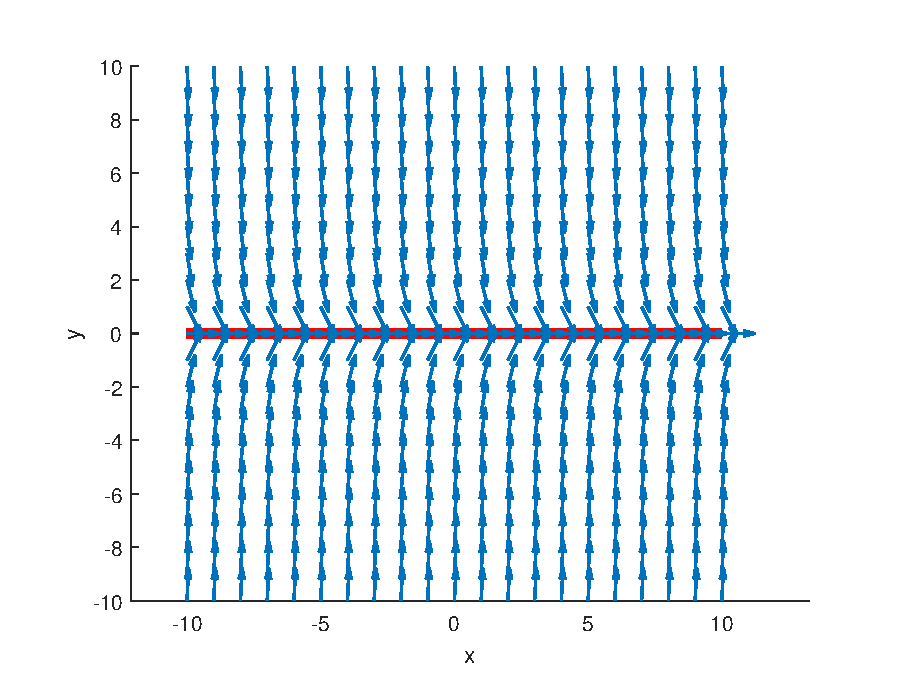
\includegraphics[width=8cm] {Figures/straightLyapunov}}
		\subfigure []{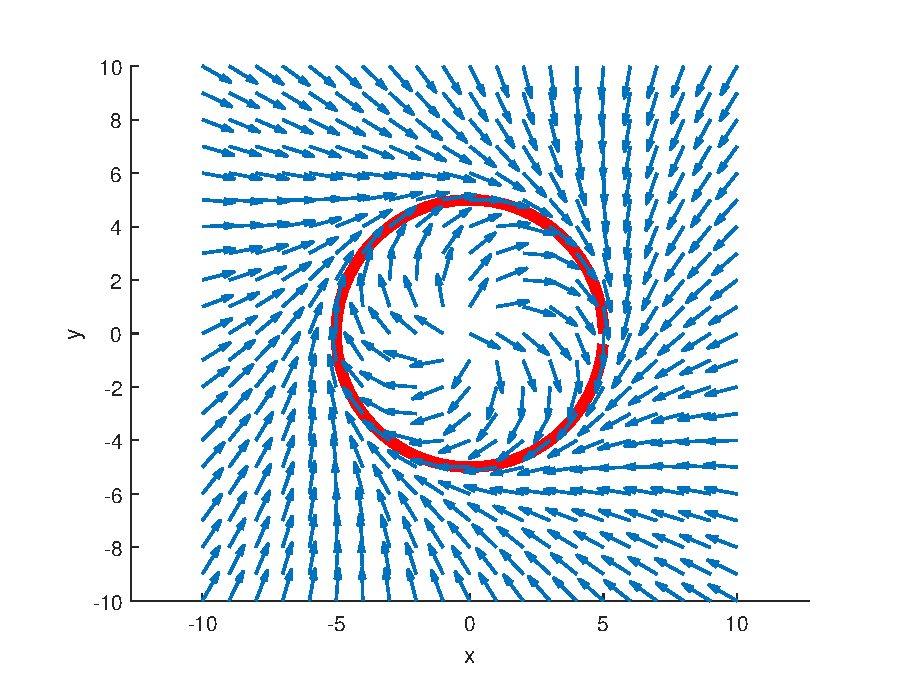
\includegraphics[width=8cm] {Figures/circularLyapunov}}
		\hspace*{0mm}
	\end{subfigmatrix}
	\caption{Vector field converging and following a) straight path b) circular path}
	\label{fig:vfPrimitives}
\end{figure}




%A circular Lyapunov vector field can be generated by the methodology described in \cite{frew_cooperative_2007}. Given the Lyapunov function:
%
%
%$y$ lateral distance from path \\
%$\chi$ difference between direction of path and course of UAV \\
%$k$ positive constant that influences the rate of transition \\
%$\chi^{\infty}$  course approach angle at large distance \\
%$\chi^{d}$ is commanded heading \\
%
%$d$ radial distance UAV from center of orbit \\
%$\gamma$ angular position with respect to orbit center \\
%$r$ orbit radius \\
%
%
%
%
%\begin{figure}[H]
%	\begin{subfigmatrix}{2}% number of columns
%		\centering	
%		\subfigure []{\includegraphics[width=7.5cm] {Figures/lineConvcirc}}
%		\subfigure []{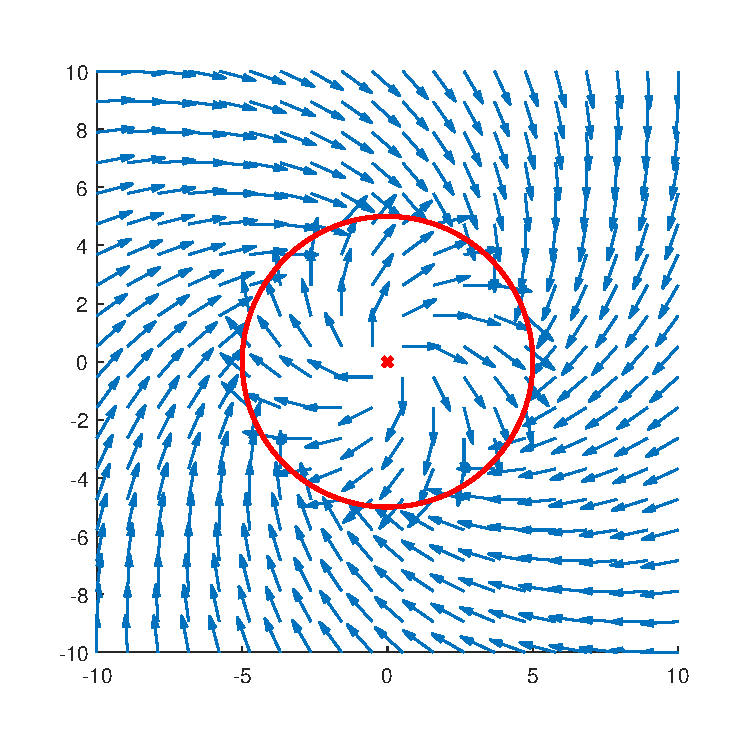
\includegraphics[width=7.5cm] {Figures/circConvCirc}}
%		\hspace*{0mm}
%	\end{subfigmatrix}
%	\caption{Vector field converging and following a) straight path b) circular path}
%	\label{fig:vfPrimitives}
%\end{figure}
%
%
%\begin{equation}\label{eq:lyapunovfunction}
%V(x,y) = (r^2 - r_d^2)^2
%\end{equation}
%where $r$ is given by the equation
%\begin{equation}
%r = \sqrt{x^2+y^2}
%\end{equation}
%and the total time derivative of Equation \ref{eq:lyapunovfunction} is
%\begin{equation}\label{eq:totaltimederivative}
%\dot{V}(x,y) = \nabla{V} \cdotp [\dot{x},\dot{y}]^{T}
%\end{equation}
%Utilizing the following equation to select the desired relative velocity $\dot{x}$ and $\dot{y}$
%\begin{equation}
%\overrightarrow{V}_{Lyapunov}\!=\!\begin{bmatrix} \dot{x_d} \\ \dot{y_d} \end{bmatrix}\!= \alpha\!\left(\dfrac{-v}{r}\right)\!\begin{bmatrix} x \dfrac{r^2-r_d^2}{r^2+r_d^2} + y \dfrac{2 r r_d}{r^2+r_d^2} \\[12pt] y \dfrac{r^2-r_d^2}{r^2+r_d^2} - x \dfrac{2 r r_d}{r^2+r_d^2} \end{bmatrix}
%\end{equation}
%and assuming $\alpha$\,=\,1 and $r$\,=\,1, the final Lyapunov VF equation is generated:
%\begin{equation}\label{eq:lyapunovvf}
%\overrightarrow{V}_{Lyapunov} = \frac{v}{r^2+r_d^2} \begin{bmatrix} - x (r^2-r_d^2) - y (2 r r_d) \\[6pt] - y (r^2-r_d^2) + x (2 r r_d) \end{bmatrix}
%\end{equation}

Straight and circular path vector fields can be selectively activated throughout flight to form more complex paths, shown in \cite{nelson_cooperative_2005,nelson_vector_2006,nelson_vector_2007,jung_unmanned_2016}. Lyapunov vector field for curved path following was presented in \cite{griffiths_vector_2006} which may allow for more complex paths and eliminates the need to switch between vector fields. \\

The Gonvalves Vector Field (GVF) method produces a similar field, however has several advantages over LVFs. GVF produces an \textit{n}-dimensional vector field that converges and circulates to both static and time varying paths. Additionally, convergence, circulation, and time-varying terms that make up the GVF are decoupled from each other allowing for easy weighting of the total field. GVFs converge and circulate at the intersection, or level set, of $n-1$ dimensional implicit surfaces ($\alpha_i:\mathbb{R}^n\rightarrow\mathbb{R} | i=1,...,n-1$). The integral lines of the field are guaranteed to converge and circulate the level set when two conditions are met: $1)$ they are positive definite and $2)$ have bounded derivatives. Consider the space with dimensions in set \textbf{q}:

%The Goncalves Vector Field (GVF) method for producing vector fields has several advantages over the Lyapunov vector field generation methods.


\begin{equation}
\mathbf{q} = \begin{bmatrix} x_1, x_2, ..., x_{n}\end{bmatrix}
\end{equation}

The total vector field $\overrightarrow{V}$ is calculated by:
\begin{equation}\label{eq:GVF}
\overrightarrow{V} = G \nabla V + H \wedge_{i=1}^{n-1}\nabla_q\alpha_i  - LM(\alpha)^{-1} a(\alpha)
\end{equation}

or in component form:

\begin{equation}\label{simpleGVF}
\vec{V} = \vec{V}_{conv} + \vec{V}_{circ} + \vec{V}_{tv} 
\end{equation}	

where $\vec{V}_{conv}$ produces vectors perpendicular to the path, $\vec{V}_{circ}$ produces vectors parallel to the path, and $\vec{V}_{tv}$ is a feed-forward term that produces vectors accounting for a time varying path. 

Convergence is calculated by:

\begin{equation}
% Total field with Conv, Circ, and Time
\vec{V}_{conv} = G \nabla V  
\label{convOnly}
\end{equation}

where scalar $G$ is multiplied by the gradient of the definite potential function $V$:

\begin{equation}
V = -\sqrt{{\alpha_1}^2 + {\alpha_2}^2}
\end{equation}



Circulation is calculated by taking the wedge product of the gradient:

\begin{equation}
% Total field with Conv, Circ, and Time
\vec{V}_{circ} =  \wedge_{i=1}^{n-1}\nabla_q\alpha_i 
\label{circOnly}
\end{equation}

In the case of $(n=3)$ the wedge product simplifies as the cross product:

\begin{equation}
% Total field with Conv, Circ, and Time
\vec{V}_{circ} =  \nabla_q\alpha_1 \times \nabla_q\alpha_2 
\label{circOnlySimp}
\end{equation}

The feed-forward time-varying component is calculated by:
\begin{equation}
\label{tv}
\vec{V}_{tv} = M^{-1}a
\end{equation}

where,

\begin{equation}
\label{mMatrix}
M =\begin{bmatrix}
\nabla\alpha_1^T \\
\nabla\alpha_2^T \\
(\nabla\alpha_1 \times \nabla\alpha_2)^T
\end{bmatrix}
\end{equation}

\begin{equation}
\label{aVector}
a =\begin{bmatrix}
\frac{\partial \alpha_1}{\partial t} \quad   \frac{\partial \alpha_2}{\partial t} \quad   0
\end{bmatrix}^T
\end{equation}

Intersecting two flat planes $(\alpha_1 = z,\alpha_2 = x)$ produces a GVF that converges and circulates a straight path, shown in Figure \ref{fig:GVFLine}. A circular path can be produced by intersecting a plane and a cylinder $(\alpha_1 = z,\alpha_2 = x^2+y^2-r^2)$.

\begin{figure}[H]
	\begin{subfigmatrix}{2}% number of columns
		\centering	
		\subfigure []{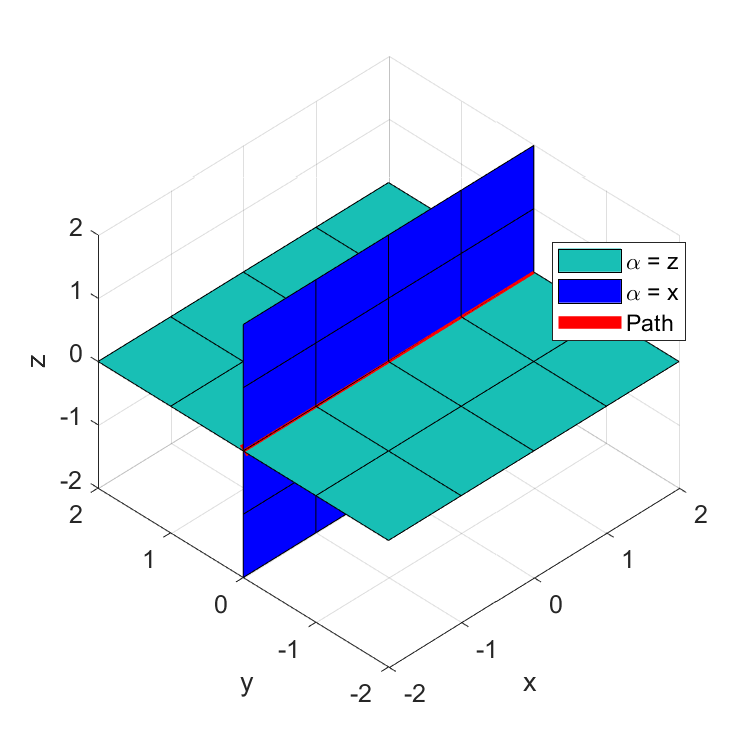
\includegraphics[width=8cm] {Figures/planeIntersection}}
		\subfigure []{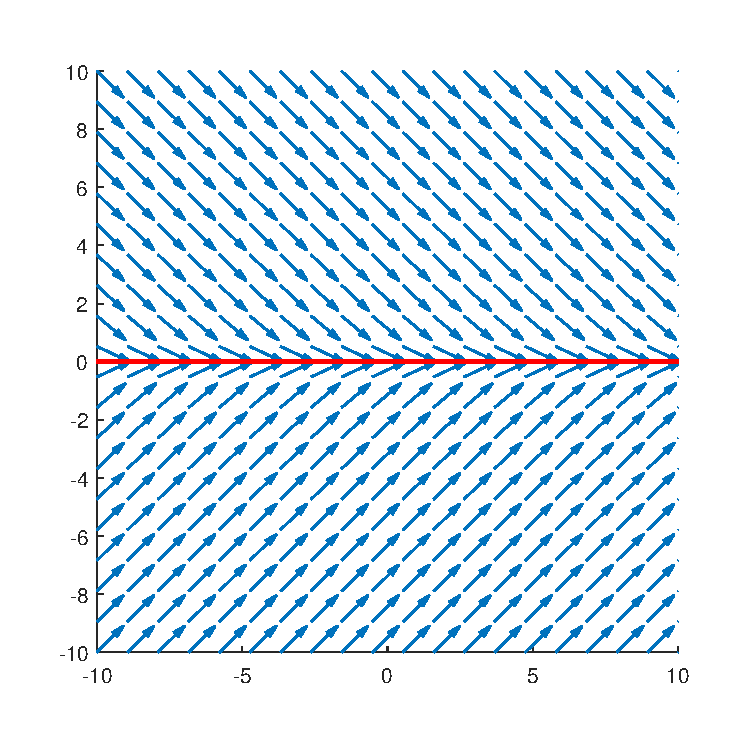
\includegraphics[width=8cm] {Figures/lineConvCirc}}
		\hspace*{0mm}
	\end{subfigmatrix}
	\caption{GVF converging and circulating straight path}
	\label{fig:GVFLine}
\end{figure}


\begin{figure}[H]
	\begin{subfigmatrix}{2}% number of columns
		\centering	
		\subfigure []{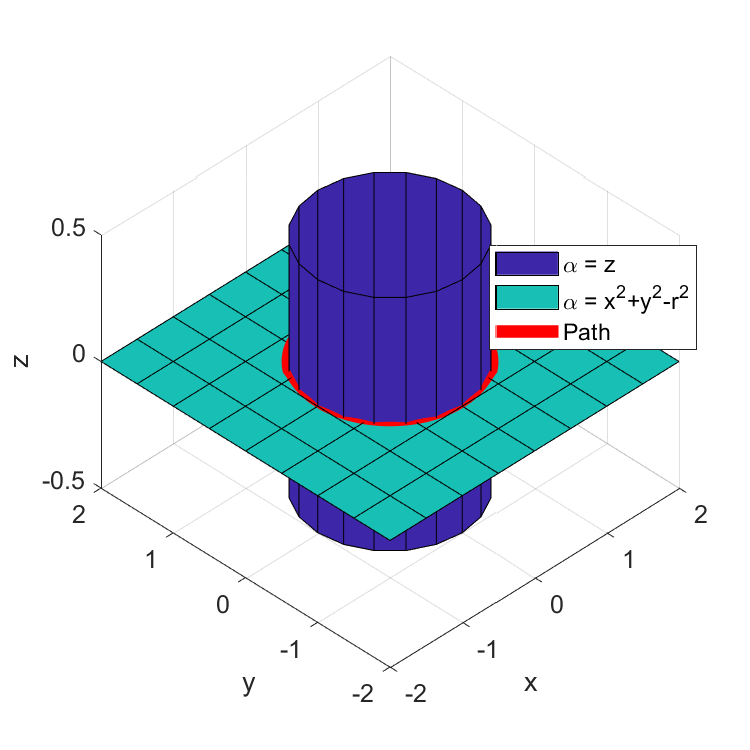
\includegraphics[width=8cm] {Figures/cylinderIntersection}}
		\subfigure []{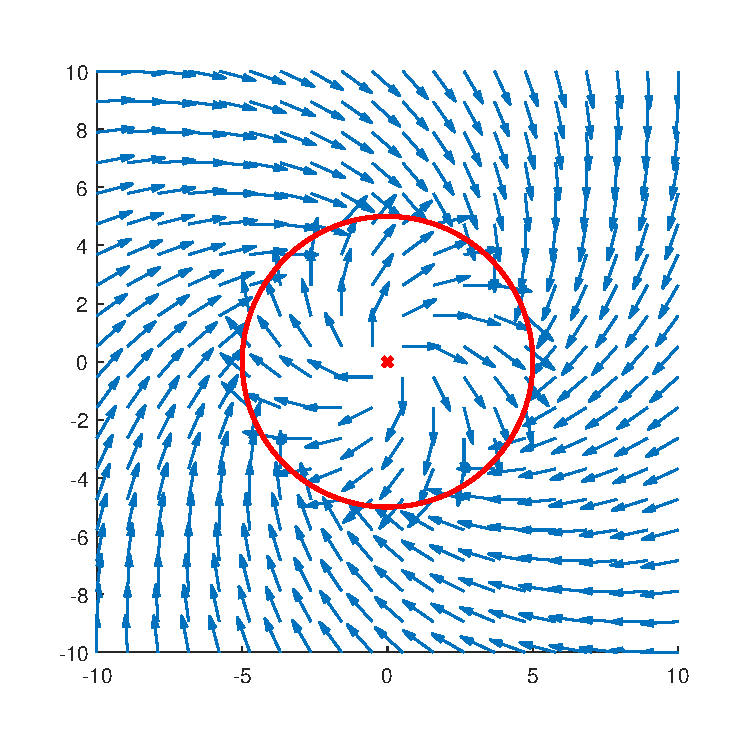
\includegraphics[width=8cm] {Figures/circConvCirc}}
		\hspace*{0mm}
	\end{subfigmatrix}
	\caption{GVF converging and circulating circular path}
	\label{fig:GVFLine}
\end{figure}

%The Goncalves method produces an \textit{n}-dimensional vector field that converges and circulates a static or time-varying path defined by \textit{(n-1)} implicit surfaces ($\alpha_i:\mathbb{R}^n\rightarrow\mathbb{R} | i=1,...,n-1$). The surface functions can represent any shape as long as they satisfy the two conditions that $1)$ they are positive definite and $2)$ have bounded derivatives. Consider the space with dimensions in set \textbf{q}:



The standoff tracking scenario presented in [Wilhelm] tasked a fixed wing UAV with loitering around a moving ground target while adding obstacle avoidance constraints. A circular attractive vector field was attached to a moving ground target. Repulsive vector fields centered at the obstacles and weighted by hyperbolic tangent decay functions were summed with the attractive circular field to produce a target loitering and obstacle avoidance guidance. The performance of Lyapunov \cite{frew_cooperative_2007} and gradient vector field \cite{goncalves_artificial_2009,goncalves_circulation_2010,goncalves_vector_2010} were compared for their cross track error with respect to the loiter circle. Gradient vector field had favorable performance due to compensation for a time-varying vector field. The gradient vector field technique also has the benefit of decoupled weighting parameters for convergence, circulation, and time-varying terms, allowing for easy modification of field behavior. \\

Decay functions for avoidance fields were investigated in [Zhu] for obstacles present on a straight path. When summing attractive and repulsive vector fields there is the possibility of guidance singularities, where magnitude and direction are equal and opposite. The presence of singularities were not addressed in [Wilhelm] and [Zhu], mentioned briefly in \cite{nelson_cooperative_2005} and observed in \cite{panagou_motion_2014}. For fixed wing UAVs the lack of guidance may prevent the UAV from avoiding an obstacle, while multi-rotor UAVs may end up in a trap situation. Singularities may be present at any location where a goal field and obstacle field are of equal strength. \\



%--- Path planning and waypoint navigation ----
%
%- Path that meets mission requirements
%- Conventionally build from straight lines connecting waypoints
%- Guidance algorithm direct the UAV towards the waypoint and switches once within a pre-determined range to the next waypoint
%
%- The UAV is not guaranteed to follow the path connecting waypoints perfectly, therefore more detailed paths require a more dense clustering of waypoints
%
%[ Figure] 
% - Sketch of waypoints, UAV following waypoints, Obstacle with waypoints placed closely together to form path around obstacle 
% 
% - Transition into potential field methods





% - Potential field is a method based on a gradient descent
%- Start at a high potential
%- End in a stable low potential
%- Obstacle represented by high potentials
%
%- Potential field combines path planning, trajectory planning, and control into a single process
%- pointed out in []
%
%- And has been used as the means for path planning in 
%- List potential field papers
%
%- Major drawbacks to potential field is the likely encounter of local minima, oscilations, etc [KandB].
%- Solutions to local minima
%
%- Object clustering (thesis document)
%- Navigation functions (thesis document)
%
%and oscillations
%- Tang (Novel potential field method)
%- Li (An Efficient Improved APF based regression search method for robot path planning)



%--- Transition to Vector Field ----
%- Such path following can be accomplished with vector fields which are a continuous source of guidance for converge to and following paths.
%
%--- Start of VF ---
%
%- Sujit compared vector field guidance to other guidance laws in [] and found that
%	- robust against wind disturbances
%	- Low cross track error
%	
%- VF produced for straight line and circular arc primitives in [Nelson]
%- Method expanded in [Griffiths] for VF following curved paths
%- Circular fields modified for standoff tracking in 
%	- frew
%	- another
%	- Wilehlm
%
%
%- Standoff tracking of a moving ground target while avoiding obstacles was presented in [Wilhelm]
%	- Fixed wing UAV tasked with tracking a moving ground target
%    - Circular attractive vector field guided UAV to track ground target while compensating for ground target velocity
%    - Repulsive vector field centered at obstacles and weighted by a hyperbolic tangent decay function
%    - Fields summed together to produce a combined guidance
%    - Two methods compared, Lyapunov and Goncalves
%    - Goncalves lower tracking error due to accounting for time varying nature of target
%    
%
%- Activation / decay functions for obstacles were investigated in [Zhu]
%
%- Singularities produced when summing together attractive and repulsive fields
%	- mentioned in [nelson] "deadzones, sinks, singularities"
%	- Observed in Panagou
%	- Expected at any VF location where an attractive field and obstacle field are of equal strength
%
%- VF use existing path planning methods to generate a guidance that minimizes distance to a path while also avoiding obstacles and singularities in obstacle fields
%---- Final Contribution ----
%
%
%
%	
%\begin{itemize}
%	\item UAS consists of vehicle, autopilot, ground station, radios
%	\item Missions typically pre-planned on ground station where flyable and obstacle free paths can be generated. (Figure of conventional waypoints)
%	\item Waypoints are sent to the autopilot over a radio and received and interpreted by the vehicles autopilot
%	\item Autopilot responsible for navigating waypoints while maintaining vehicle stability
%	\item Due to turn rate constraints or external disturbances, a vehicle may not follow the path perfectly where it may encounter an obstacle previously planned for
%	\item Demonstrate the above with dubins
%	\begin{itemize}
%		\item Introduce dubins as a way to approximate a UAVs dynamics, assume control working (cite)
%		\item Equations
%		\item Demonstrate Dubin's UAV not perfectly following path
%		\item Demonstrate Dubin's with wind not following path
%	\end{itemize}
%\end{itemize}
%
%
%
%\begin{itemize}
%	\item Reduced error for straight line and circular path following has been achieved by using vector field guidance (sujit)
%	\item Continuous vectors that asymptotically converge and follow straight and circular paths are both robust and produce guidance that results in low cross track error
%	\item Lyapunov VF primitives introduced (Nelson). Nelson stitched together primitives to produce complex paths similar to navigating waypoints
%	\item Curved path vector field was introduced in (griffiths)
%	\item Goncalves VF
%	\begin{itemize}
%		\item Path of any shape
%		\item Accounts for TV nature of paths
%		\item Field is produced by summing convergence and circulation terms that are easily accessable
%		\item Integral lines guaranteed to converge
%	\end{itemize}
%	\item Obstacles considered in standoff tracking scenario Wilhelm
%	\begin{itemize}
%		\item TV field loiter around moving ground target
%		\item obstacles represented by repulsive field 
%		\item Did not consider or identify singularities present in summed fields
%		\item Singularities are small regions or wells of no guidance where UAV may be trapped
%		\item No information on how to go around obstacle
%		\item Field used as a high level specification for avoidance
%		\item Hyperbolic activation function
%	\end{itemize} 
%
%	\item Activation functions of obstacle avoidance investigated in Zhu
%	\item Determining VF parameters that influence performance and singularity location 
%\end{itemize}
%
%
%
%
%
%\section{Methodology}
%\subsection{Singularity Detection}
%\begin{itemize}
%	\item Present VF equations for straight path following
%	\item Present VF equations for circular obstacle and obstacle definitions
%	\begin{itemize}
%		\item Repulsion, small 'path' radius
%		\item Decay function
%		\item No circulation versus circulation (side by side figure)
%	\end{itemize}
%
%	\item Sum fields together and show stages of normalization
%	\item Identify pre normalization singularity
%	\begin{itemize}
%		\item Surface plot (x,y,magnitude)
%		\item Identify undefined region and singularity (Evaluating entire space)
%		\item Find minimum of guidance function by evaluating several initial conditions
%		\item Method for finding all singularities as a reference to future look-ahead methods
%	\end{itemize}
%
%
%	\item Look-ahead and singularity detection
%	\item Location of all singularities not important if UAV is not going to encounter them
%	\item Introduce UAV flight envelope
%	\item Time, turn rate, constant velocity, produces possible locations of UAV
%	\item Evaluate ICs on flight envelope when near obstacle
%\end{itemize}
%
%\subsection{Modifying VF to avoid singularities}
%\begin{itemize}
%	\item Cause and location of singularities
%	\begin{itemize}
%			\item Adding circulation to the repulsive obstacle field reduces /removes singularity
%			\item Singularities will occur where both fields have equal strength
%			\item Prediction of singularity location based on decay function
%	\end{itemize}
%
%	\item Side by side repulsion and repulsion+circ singularity locations
%	\item Singularity detected, modify field to remove singularity from flight envelope
%	\item Objective function is:
%	\begin{itemize}
%		\item Avoid obstacle 
%		\item Avoid singularities
%		\item Minimize deviation from path
%	\end{itemize}
%
%\end{itemize}
%
%\section{Simulation}
%\begin{itemize}
%	\item Dubins UAV following a pre-planned straight path
%	\item Obstacle encountered
%	\item A guidance solution must be determined that:
%	\begin{itemize}
%		\item Determines location of singularities if present (inside flight envelope)
%		\item Solve VF parameters to remove / mitigate singularities
%		\item Solve VF parameters that result in guidance that  minimize error from path
%	\end{itemize}
%
%	\item Various UAV speeds
%	\item Worse case scenario presented (on path)
%	\item Multiple obstacles on path (sequential)
%	\item Compare non-modified guidance with modified guidance
%	\begin{itemize}
%		\item Deviation from path
%		\item Yes/no obstacle avoided
%		\item singularity avoided in flight envelope
%	\end{itemize}
%\end{itemize}


\section{Conclusion}



\section*{Appendix}



\section*{Acknowledgments}

\bibliography{bib}

\end{document}
